\chapter{Evaluation and Analysis}\label{sec:results}

The scripts that perform the evaluation of our testing set, are \texttt{evaluation.sh} and \texttt{exec\_query.sh}.

\section{Video Identification}
After receiving a list of matching windows from the KD-Tree, we classify each one of them as a proper \textbf{match} iff the window's ID matches the ID of the capture we passed to the Java identification process, whereas, if the ID of the capture and the window ID are different, we classify the returned window as a \textbf{mismatch}.

We then report, for various $\omega$ window sizes, the accuracy of our method, to be the proportion of matches with respect to the number of mismatches over the total number of returned windows as:

Let $n$ be the number of returned windows for a given capture trace, and let $TP$ represent the number of matches, and $FP$ to represent the number of returned mismatches:

It follows that $n = TP + FP$

\begin{equation*}
    acc = \dfrac{TP}{n} = 1 - \dfrac{FP}{n}
\end{equation*}

As mentioned in \Cref{sec:testing}, our testing dataset consists of the same 100 movies present in the database at 8 unseen enforced bandwidths. We pass each capture to the identification process, that runs the evaluation by varying the window size $\omega$, and the corresponding key size $\kappa$. For every run, we then compute the number of matches/mismatches, and report the statistics shown in \Cref{lst:stats}. In addition, we plot for each configuration the number of matches, the number of collisions and the number of mismatches. The number of collisions, represents the number of matches from different bandwidth levels, (e.g. suppose to have a capture at 6.0 \emph{Mbps}, now assume the KDTree returns as matching windows, a list of matches all of the same movie, but at different bandwidths, 5.0 \emph{Mbps}, and 7 \emph{Mbps}, then the number of collisions is 2).

%\begin{figure}[!h]
  %\centering
  %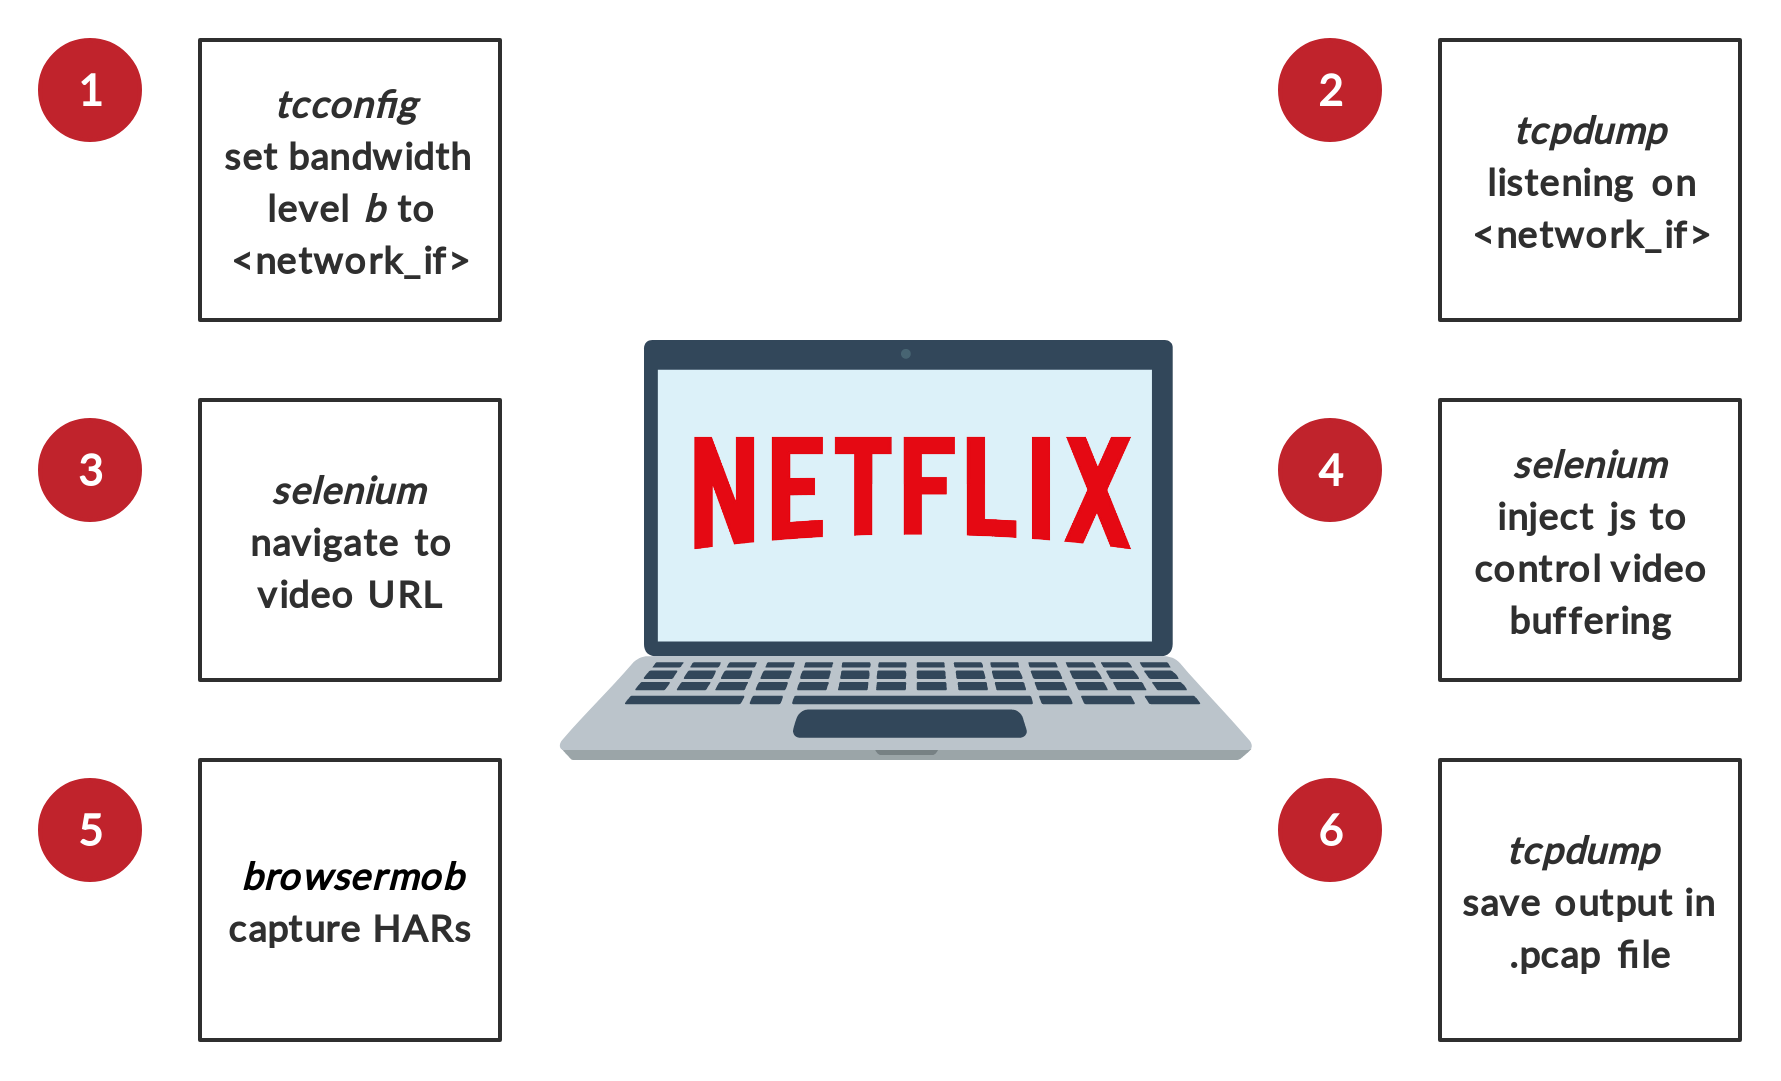
\includegraphics[width=\columnwidth]{img/fingerprints.png}
  %\caption{Overview of the process of acquiring video fingeprints.}
  %\label{fig:fingerprints}
%\end{figure}

\section{Bitrate Ladders}

At first, we evaluate the accuracy of the reconstruced bitrate ladders by computing the RMSE between each one and its corresponding HAR-based bitrate ladder. We have decided to use the RMSE, as it is a well-known indicator that aggregates the residuals to give a measure of the magnitude of error in our predictions, and it is computed as follows.

Let $Y=\{y_1, y_2 \dots y_n\}$ be the set of HAR-based bitrates for movie $m$, at enforced bandwidth
$b$, and let $\hat{Y}=\{\hat{y}_1, \hat{y}_2 \dots \hat{y}_n\}$ be the set of ADU-based computed bitrates for the same
movie at the same enforced bandwidth, then:

\begin{equation*}
    RMSE_{m, b} = \sqrt{\dfrac{\Sigma_{i=0}^{n}(y_i - \hat{y}_i)^2}{n}}
\end{equation*}

where $n = |Y| = |\hat{Y}|$

Then, the \emph{mean-normalized} RMSE is given by:

\begin{equation*}
    NRMSE_{m, b} = \dfrac{RMSE_{m, b}}{\overline{\hat{y}}}
\end{equation*}


